\section{Introduction}
\subsection{Background}

For the last few decades, the global energy landscape has been undergoing a significant transformation, driven by climate change and the need to reduce greenhouse ges emissions in order to reduce its impact. Europe has been at the forefront of this transformation with \textcolor{red}{CITE EXAMPLES OF EUROPEAN WORK} and Spain, as its fifth largest economy has had a significant part in this. In fact, Spain has shown drive of its own by being at the forefront of many of these initiatives with a robust commitment to renewable energy sources, like with \textcolor{red}{SPAIN EXAMPLES}. This country has set ambitious targets for renewable energy integration, seting a target of having 74\% of its energy coming from renewable generation facilities by 2030 and a 42\% share of renewables in energy end use, as per the 2021 Spain Energy Policy Review \cite{energy_policy_review_spain_2021}. Spain is particularly well positioned for this transition due in part to its favourable geographical conditions. Being one of the southermost parts of Europe with a mediterranean climate allows for long periods of intense sunshine, and its extensive coast also provides good conditions for regular and powerful wind. 

Like any other industrialised country, historically Spain has relied heavily on fossil fuels. The recent growth of renewable energy has been driven by several factors, including technological advancements, a reduction in costs driven by the economies of scale in production mainly in China and by government policies. Amongst these policies, the first big push came from the Royal Decree 661/2007 through which the production of renewable energy in Spain was regulated \cite{boe_661_2007}. In this legislation, a premium was awarded to producers of renewable energy in order to incentivize investment in the sector. However, as soon as 2010 these premiums started to be reduced due to the general deficit in the sector and the financial constraints imposed on the state by the 2008 financial crisis. These reductions culminated in 2013 with a drop in 40\% of all premiums available at that point. This led to the bankruptcy of a great number of companies which had invested heavily mainly in solar power plants and which relied on these subsidies for their required profitability. In 2015 the sector was further regulated through what came to be known as the "Sun Tax" \cite{boe_900_2015}. This royal decree imposed a tax on self-consumption systems -- individuals or companies installing solar PV panels to generate part of their own electricity -- in order to compensate for the additional system maintenance needed by these systems. Since then, thanks to the drop in costs these subsidies have stopped being necessary with solar energy being profitable without government intervention, and some argue even the most profitable source of energy \cite{gunther_glenk_reichelstein_2022}. This advantageous financial landscape, together with a recent regulatory push driven mainly from the European Union, has prompted a new golden age of investment in renewable energy in Spain. In \autoref{fig:investment-clean} the growing trend in investment can be clearly seen, except for the drop in 2021 created by the Covid-19 crisis. 

\begin{figure}[ht]
    \centering
    \captionsetup{justification=centering}
    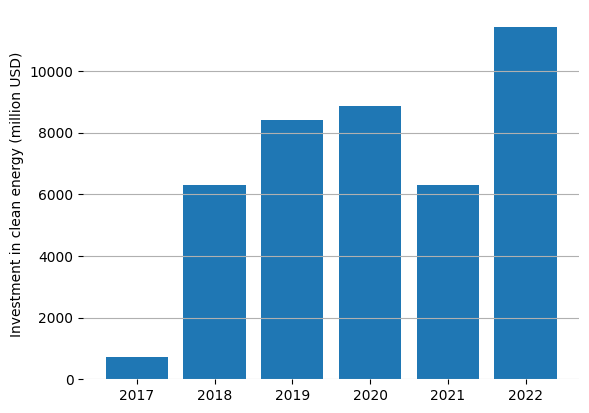
\includegraphics[width=0.7\linewidth]{assets/investment-clean.png}
    \caption{Investment in the Spanish clean energy sector, in million USD. \cite{renewable_energy_investments_2022}}
    \label{fig:investment-clean}
\end{figure}

This showcases the obvious interest there is in renewable energy in general in Spain. However, when talking about renewable energy it is very important to outline the different renewable energy resources and their corresponding technolgies \cite{ellabban_haitham_blaabjerg_2014}:
\begin{itemize}
    \item \textbf{Biomass}: Biomass energy is derived from organic materials, mainly plant and animal matter such as wood, agricultural crops, waste, and algae. It can be burned directly to produce heat and power a thermal power plant or it can be converted into biofuels like bioethanol or biodiesel. These fuels are then used in thermal power plants or for other uses like vehicle powering. It is very versatile with many of the main benefits of fossil fuels and can be used to reduce waste. However, sustainable sourcing of the biomass is critial, as otherwise it can lead to deforestation or other environmental issues.
    \item \textbf{Geothermal}: Geothermal energy harnesses the higher and more constant temperatures found deep below the Earth's surface, which originates from the planet's hot core due to the high pressure and the radioactive decay of different materials. Geothermal plants directly source hot water from underwater sources or pump fluids deep into the surface, heating it and retrieving it afterwards. This hot fluids can be used in a thermal power plant, as part of the cycle to preheat the working fluid or directly to heat up some buildings. It provides a constant and reliable energy supply not dependent on weather conditions and it has a samll land footprint. However, it is very location-specific, working best in regions with significant tectonic activity and with easily drillable materials in the ground. 
    \item \textbf{Hydropower}: Hydroelectric power is the power of flowing water. This water is generally stored in a dam and released to flow through turbines which generate electricity, although other systems which do not require dams and use water flowing in rivers are also possible. Worth mentioning are also pumped storage plants, which although are not strictly a renewable energy resource can be used as energy storage systems. Hydroelectric power has high efficiency and can provide electricty on demand with very short warm up periods, however the initial investment to build the dam is very costly, it cannot be placed anywhere and can disrupt the local ecosystems.
    \item \textbf{Marine}: Marine power leverages different sources of energy available in the seas and oceans. There are six main energy sources within this category:
    \begin{itemize}
        \item Wave: It transforms the kinetic energy of waves in their up and down movements into electrical energy.
        \item Tidal range: It leverages the difference in height between the high and low tide to generate electricity. 
        \item Tidal currents: It harnesses the horizontal currents caused by the rising and falling of the tide.
        \item Ocean currents: Similar to the previous source, however it leveraes currents not necessarily caused by tides, but caused by the dynamics of the ocean.
        \item OTEC: Ocean thermal energy conversion exploits the temperature difference between the warmer surface water and the colder deep water as the hot and cold sources of a thermal cycle to generate electrictiy.
        \item Salinity gradients: It leverages the difference in saline concentration between different areas of the ocean.
    \end{itemize}
    Many of these energy sources are still undergoing intensive research and developement and are still in the prototype and demonstration stage.
    \item \textbf{Solar}: Solar energy leverages the energy of solar radiation reaching us from the sun in several different ways:
    \begin{itemize}
        \item Photovoltaic: Solar PV systems directly convert the energy of the photons sent by the sun into direct current through the photoelectric effect \cite{einstein_1905}. The PV cells, generally made out of silicon, have an efficiency of around ~20\%. However they are very modular and can be produced at scale, helping achieve the tremendous drop in cost that has been seen during the last decade. 
        \item Thermal: Solar thermal power leverages the heating capacity of the solar radiation to harness its power. Although it is often used to directly heat up buildings, it can also be used to generate electricity. Concentrating solar power (CSP) produces electricity by concentrating the solar irradiance through mirrors and lenses to heat a liquid which is used in a thermal power cycle. 
    \end{itemize}
    \item \textbf{Wind}: Wind energy refers to the kinetic energy of wind currents. This energy can be transformed through wind turbines into electrical energy. Wind power is generally obtained through two different types of setups. There are on-shore and off-shore power plants, with the former being installed in land and the latter in seas or oceans near the coast. Off-shore installations have some advantages, like more powerful and constant wind, no land erosion and less landscape visual degradation, however its installation is more costly. 
\end{itemize}

As it can be seen, there are many different renewable energy resources and technologies that can be used to harness them and aid in the energy transition. However, not all of them are equivalent, with different technologies having different levels of maturity, profitability, capital requirements, etc. That is why generally the renewable energy mix is not very uniform. 

\begin{figure}[ht]
    \centering
    \captionsetup{justification=centering}
    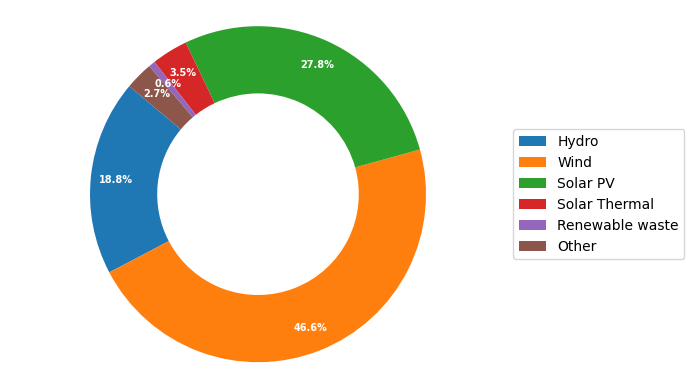
\includegraphics[width=0.7\linewidth]{assets/generation-mix.png}
    \caption{Generated renewable electricity mix in Spain in 2023. \cite{renewable_generation_reports_2023}}
    \label{fig:generation-mix}
\end{figure}

In \autoref{fig:generation-mix} it can be seen how solar, wind and hydro energy covers more than 95\% of the energy generation of 2023 -- as percentage of the total generation of 134.321 GWh of renewable energy -- while other sources like geothermal and biomass are almost negligible. 

\subsection{Motivation}
\label{sec:motivation}

In the previous section in \autoref{fig:generation-mix} a promising picture of the renewable energy generation in Spain could be seen, even more when the total generation is compared with the non-renewable generation of 132.486 GWh in Spain \cite{renewable_generation_reports_2023}, showing how renewable energy generation surpassed the 50\% mark.

However, the generation mix shown is also a source for concern. A 77.9\% of the total energy mix was produced through solar and wind energy. Solar and wind energy share some characteristics which lead to some grave challenges to the overall electrical system. Mainly, these characteristics and consequent challenges are:
\begin{itemize}
    \item \textbf{Variability}: These energy sources are intermittent. That is, one cannot choose to turn on a solar power plant at any moment, as its output depends on the solar input, which cannot be decided by the operator. This is translated into a very variable pattern of generation with high peaks and low troughs. 
    \\This variable pattern of production with rapid ramps leads to the need of having other power plants with also rapid ramp ups which can step up after a sudden fall of solar or wind production. These other plants also need to be very flexible to adapt to the wide changes in generation from these renewable resources.
    \item \textbf{Uncertainty}: Not only can these technologies not be discretionarily dispatched, but often it is difficult to know in advance what their behaviour will be at some point in the future. The further out into the future one looks, the less certain the sun and wind forecasts become, and thus the less certain the production output forecasts become.
    \\Many of the problems of variability are accentuated by the fact that this variability is uncertain. Given the grid players are uncertain about the renewable generation, large reserves need to be allocated in case the prediction fails. This in turn leads to more expensive electricity for the end consumer if the same level of reliability is required. 
    \item \textbf{Location specific}: The renewable resources are often geographically concentrated. For example, sun is more prominient in the south of Spain and wind around the coast. 
    \\Having many of these power plants geographically concentrated leads to several problems when all of them are producing at high outputs at the same time. Power lines connecting the renewable rich area with the rest can become overloaded forcing shutdowns and cutoffs. Furthermore, great voltage differences between areas in the grid can appear.
    \item \textbf{Generator technology}: The induction generators generally used in wind turbines or the inverters in solar power plants behave differently to the synchronous generators used in thermal power plants, which leads to problems in frequency control as will be outlined below. 
    \\This difference in generator technology leads to several problem. The first one being that these power plants are unable of providing the primary reserve matching supply and demand at the expense of frequency changes that synchronous generators supply automatically. Furthermore, these generators do not provide the same reactive power supply as the synchronous generators, and in the case of induction generators in wind turbines they in fact consume reactive power in order to function. It has also been hypothesized how these generators can lead to angular instability \cite{vittal_raja_ayyanar_2023}. The generators of wind turbines have also been shown to lead to problems of power quality due to the injection of different harmonics \cite{muljadi_butterfield_chacon_romanowitz_2006}. 
    \item \textbf{Low capacity factor}: Due to the variability in the resources, the capacity factor of installations leveraging sun and wind is generally lower to that of other non renewable technologies. 
\end{itemize}

Even more importantly, the greater the share of overall energy that comes from solar and wind sources the more pronounced these challenges will become. For more details regarding these characteristics and their consequences, refer to \cite{ahmed_fahad_2020}, \cite{kumar_pandey_sinha_2016} and \cite{steen_goop_2014}.

Grid operators need to consider these challenges at a short and medium term when opperating the grid, and plannificators should also consider it when planning the long term of the grid. 

The first two characteristics, the variability and uncertainty of these resources, leads in fact to a great problem in long term planning. When deciding where to locate which power plants and of what capacity, it is important to have accurate models of all resources. In fact, many of the optimization models used in long term planning require forecast models of these resources, which is very challenging due to the aforementioned characteristics. The lack of realistic and accurate models of solar and wind energy generation is precisely what this work aims to solve.

\subsection{Objective and scope}
\label{sec:objective-and-scope}
By looking at the overview of the wind and solar energy presented in \autoref{sec:motivation} \nameref{sec:motivation} and understanding the objectives and challenges of grid planners -- long term distribution of resources to ensure the grid's effectiveness and reliability -- the need for a model that can be used by these planners has become apparent. 

To be more precise, for such a model to be useful it must accurately represent the wind and solar energy generation marginal and joint distributions. The characteristics the model must fulfill are the following:
\begin{itemize}
    \item \textbf{Modeled variable}: The variable to be modeled is the hourly capacity factor of wind, solar PV and solar thermal energy generation. The capacity factor $f_t$ can be calcualted as 
    \begin{equation}
        \label{eq:capacity-factor}
        f_t=\frac{E_t}{P_t t}
    \end{equation}
    Where $E_t$ is the energy generated in a given timeframe, $P_t$ is the power output rating -- that is the rated installed capacity -- and $t$ is the length of the timeframe. As it can be seen, the capacity factor is a unitless ratio. 
    
    It has been chosen as the modeled variable due to having several beneficial characteristics. Numerically, $f_t \in \left[0,1\right]$ which makes it easier to model. It also is able to show the power generation without regarding the installed capacity. The installed capacity is often determined by policy decisions, awarded licenses or discretionary investment decisions by electricity companies and is thus harder to accurately model. The capacity factor however allows for an accurate representation of the generated power. 

    The hourly frequency has been chosen as it is short enough to allow for significant changes throughout the day, but is not short enough for noise to become a significant part of the variable. Furthermore, this is the frequency used by most market players, with the electrical market quoting hourly values for example. 

    The wind, solar PV and solar thermal capacity factors have been chosen as independent variables because the three of them have significantly different driving factors, making them have different dynamics that can be captured by individual models. Even the solar PV and solar thermal have different dynamics, thanks to the inertia provided by the storage of heat in solar thermal power. 
    \item \textbf{Input variables}: The only exogenous variable that will be used in all models are the historical values of these capacity factors and temporal variables such as the month or hour. A purely time series approach has been taken, as opposed to other physical approaches that leverage weather forecasts. The intuition for this decision is that the information provided by the weather or any other significant variable should be integrated in the capacity factor, and relying on other external variables forces a two step approach where a model for those variables needs to be created and then a model for the capacity factor needs to be created, as there are no accurate forecasts for any of the other possible exogenous variables with a long enough timeframe. 
    \item \textbf{Geographical scope}: The capacity factor will be that of the national Spanish power system. 
    \item \textbf{Temporal scope}: The model should be able to forecast the capacity factor for a period of 1 to 10 years into the future, with hourly values. 
    \item \textbf{Methodological scope}: Statistical, machine learning and deep learning models will be studied as candidates to modelling this variable. 
\end{itemize}

% \subsection{Study structure}
